\documentclass{scrartcl}

\usepackage{amssymb}
\usepackage{amsmath}
\usepackage{tikz}
\usetikzlibrary{patterns}	%for hatching
\usetikzlibrary{calc}		%for centerarc

\def\centerarc[#1](#2)(#3:#4:#5)% Syntax: [draw options] (center) (initial angle:final angle:radius)
{ \draw[#1] ($(#2)+({#5*cos(#3)},{#5*sin(#3)})$) arc (#3:#4:#5); }

\begin{document}
	
	%from Althusser - Philosophy and the Spontaneous Philosophy of the Scientists, p. 164
%	\begin{figure}
%		\centering
		%\hspace{1.25cm}
	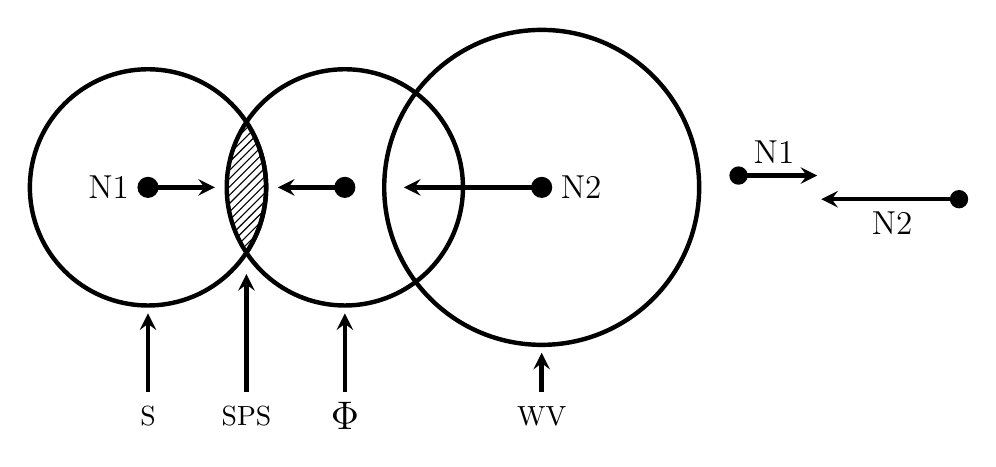
\begin{tikzpicture}[>=stealth,ultra thick]
	%circles
	\draw (0,0) circle (2cm);
	\draw (-2.5,0) circle (1.5cm);
	\draw (-5,0) circle (1.5cm);
	
	%black dots
	\filldraw (0,0) circle (3pt);
	\filldraw (-2.5,0) circle (3pt);
	\filldraw (-5,0) circle (3pt);
	%
	\filldraw (2.5,0.15) circle (2.5pt);
	\filldraw (5.3,-0.15) circle (2.5pt);
	
	%horizontal arrows
	\draw[->] (0,0)--(-1.75,0);				%rightmost
	\draw[->] (-2.5,0)--(-3.35,0);			%center
	\draw[->] (-5,0)--(-4.15,0);			%leftmost
	%
	\draw[->] (2.5,0.15)--(3.5,0.15);		%N1 = Nucleus 1
	\draw[->] (5.3,-0.15)--(3.55,-0.15);	%N2 = Nucleus 2
	
	%vertical arrows
	\draw[->] (0,-2.6)--(0,-2.1);			%WV = World-View
	\draw[->] (-2.5,-2.6)--(-2.5,-1.6);		%\Phi = Philosophy
	\draw[->] (-3.75,-2.6)--(-3.75,-1.1);	%SPS = Spontaneous Philosophy of the Scientist
	\draw[->] (-5,-2.6)--(-5,-1.6);			%S = Science
	
	%labels
	\node at (-5.5,0) {{\large N1}};
	\node at (0.5,0)  {{\large N2}};
	%
	\node at (2.95,0.45)  {{\large N1}};
	\node at (4.45,-0.45) {{\large N2}};
	%
	\node at (0,-2.9)    {WV};
	\node at (-2.5,-2.9) {{\Large $\Phi$}};
	\node at (-3.75,-2.9){SPS};
	\node at (-5,-2.9)   {S};
	
	%hatched intersection
	\clip (-2.5,0) circle (1.5cm); 			%keep only what is inside center circle
	\draw[pattern=north east lines, pattern color=black] (-5,0) circle (1.5cm);  %left circle
	%code via: http://users.ju.edu/hduong/math220/venn_diagrams.pdf
	\end{tikzpicture}
%		\caption{Representing the existence of \textit{two irradiating nuclei}}
%	\end{figure}
	
	
	\vspace{1.5cm}
	
	
	%l'avenir dure longtemps / the future lasts a long time
	%Note: on book covers, Althusser is standing in front of the rightward cap
	%I am referring to a mysterious drawing of it, contained on the following pages: 
	%http://www.faculty.umb.edu/gary_zabel/Courses/Spinoza/Texts/Radical%20Spinoza.htm
	%https://dialnet.unirioja.es/descarga/articulo/2723426.pdf (instant download)
	%
	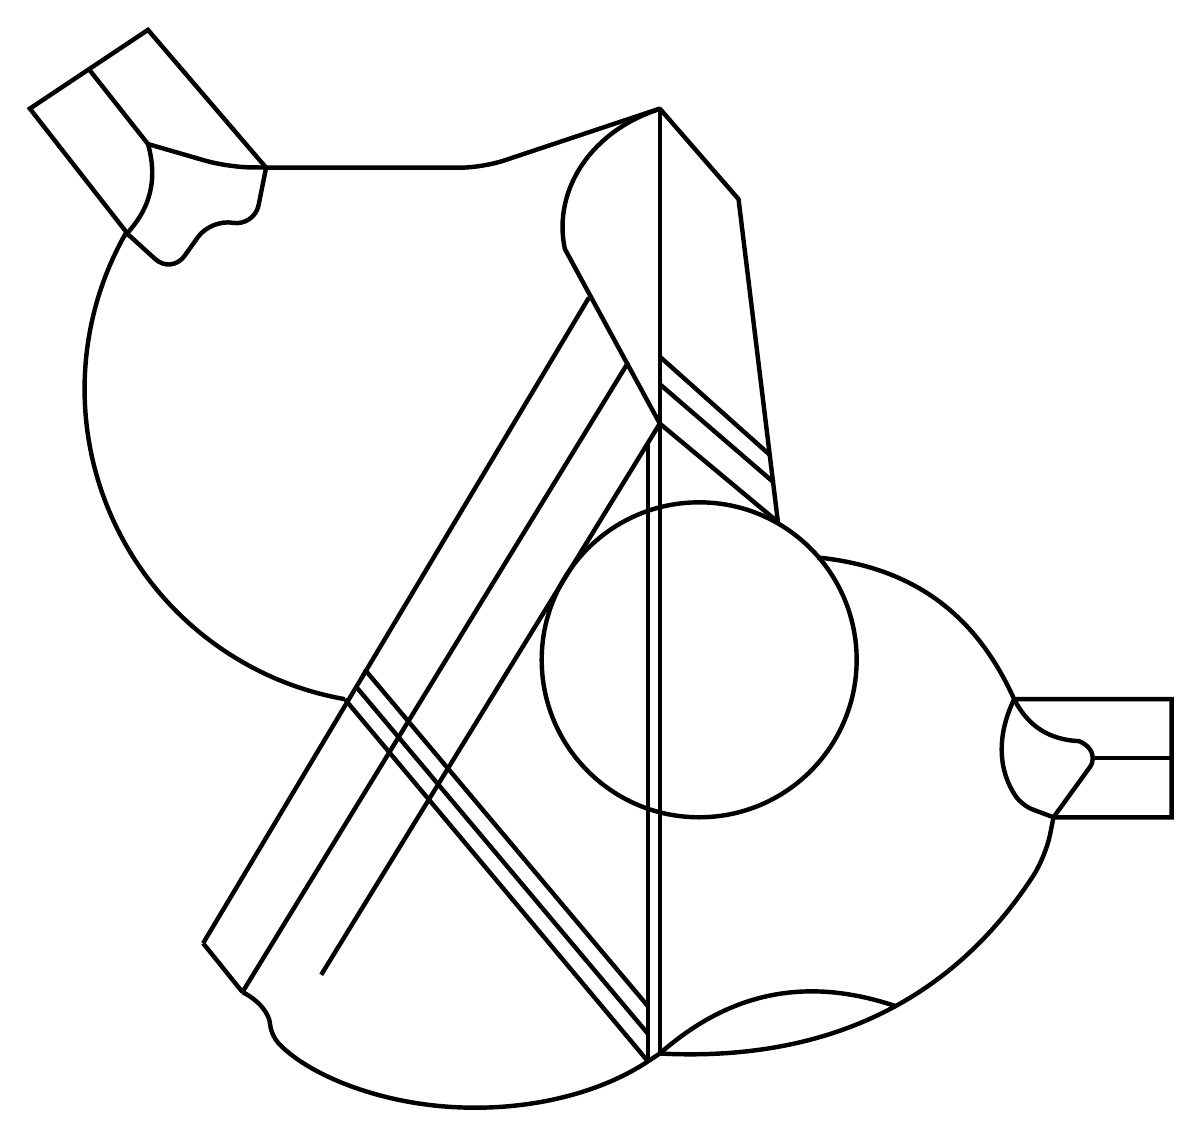
\begin{tikzpicture}[ultra thick]
	%vertical lines
	\draw (0,4)--(0,-8);
	\draw (-0.15,-0.22)--(-0.15,-8.1);
		\draw (0,-8)--(-0.15,-8.1);
	\draw (0.5,-3) circle (2);
	
	%upper-right
	\draw (0,0)--(1.5,-1.25);				%diagonal (rightward) from origin
	\draw (0,0.5)--(1.45,-0.75);
	\draw (0,0.85)--(1.4,-0.4);
	\draw (1.5,-1.25)--(1,2.85)--(0,4);		%rightward border
	
	%upper spiral
	\draw (0.015,4) arc (110:190:1.9cm and 1.6cm) -- (0,0);
	\centerarc[](-0.625,2.5)(200:360:0.625)	%top spiral
	\centerarc[](-0.58,2.5)(-45:180:0.59)
	\centerarc[](-0.72,2.55)(185:360:0.45)
	\centerarc[line cap=round](-0.55,2.5)(0:190:0.28)
		%spiral looks weird, but it's weird in the original -- not sure how to fix
	
	%NE--SW diagonals
	%\draw (0,0)--(-4.9,-8);				%diagonal (leftward) from origin; (-4.6,-7.5)
	\draw (0,0)--(-4.3,-7);					%shorter line that merges into spiral
	\draw (-0.4,0.78)--(-5.3,-7.22);
	\draw (-0.9,1.6)--(-5.8,-6.6);
	\draw (-5.3,-7.22)--(-5.8,-6.6);
	
	%SE--NW diagonals
	\draw (-0.15,-8.10)--(-4.00,-3.5);		%bottom
	\draw (-0.15,-7.75)--(-3.85,-3.35);
	\draw (-0.15,-7.40)--(-3.75,-3.12);
	
	%leftward arc
	\draw (-4.00,-3.5) arc (260:150:4cm and 4cm);
	
	%northeast cap
	\draw (-5,3.25)--(-6.5,5)--(-8,4)--(-6.75,2.4);	%cap
	\draw (-7.25,4.5)--(-6.5,3.55); 		%center line
	\draw[rounded corners=8pt] (0,4)--(-2.25,3.25)--(-5,3.25)--(-5.5,3.26)--(-6.5,3.55);
	\draw (-6.5,3.55) to[bend left] (-6.8,2.38);
	\draw[rounded corners=8pt] (-5,3.25)--(-5.15,2.5)--(-5.7,2.6)--(-6.2,1.9)--(-6.75,2.4);
	
	%bottom right
	\draw (0,-8) to[bend left] (3,-7.4);	%crescent
	\draw[rounded corners=8pt] (0,-8) to[bend right] (4.9,-5.5) -- (5,-5);
	\draw (5,-5)--(6.5,-5)--(6.5,-3.5)--(4.5,-3.5) to[bend right] (2,-1.7);
	\draw (6.5,-4.25)--(5.5,-4.25); 		%center line
	%
	\draw (5.5,-4.25) arc (0:60:0.35cm and 0.25cm) to[bend left] (4.5,-3.5);
	\draw (5.5,-4.25) arc (0:-30:0.35cm and 0.25cm) -- (5,-5); %try to round this a bit
	%
	\draw[rounded corners=4pt] (5,-5)--(4.6,-4.85) to[bend left] (4.5,-3.5); %bottom of cap
	
	%bottom left
	\draw[rounded corners=4pt] (-0.15,-8.1) arc (317:210:3cm and 1.85cm) to[bend right] (-5.3,-7.22);
	\centerarc[](-3.43,-7.5)(145:360:1)		%bottom spiral
	\centerarc[](-3.18,-7.5)(0:180:0.75)
	\centerarc[](-3.43,-7.5)(180:360:0.5)
	\centerarc[line cap=round](-3.18,-7.5)(0:180:0.25)
	
	%\node[circle,draw=red,fill=red,inner sep=0pt,minimum size=6pt] at (0,0) {}; %origin
	%\draw[help lines] (-9,-10) grid (7,6);
	\end{tikzpicture}
\end{document}
